\documentclass[12pt]{article}
\usepackage{blindtext}
\usepackage{imakeidx}
\usepackage[utf8]{inputenc}
\usepackage[T1]{fontenc}
\usepackage{enumitem}
\usepackage[obeyspaces]{url}
\usepackage{graphicx}
\usepackage{float}
\usepackage{xcolor}   % for \textcolor
\usepackage{fixltx2e}
\usepackage{hyperref}
\graphicspath{./immagini }

\title{%
  MCS 2020 \\
  \large Algebra lineare numerica \\
   Compressione di immagini tramite la DCT}

\date{21/05/2020}
\author{Silva Edoardo 816560, Zhigui Bryan 816335, Marchetti Davide 815990}
\makeindex

\begin{document}
\maketitle

\section{Abstract}

	Si vuole presentare un software che implementa una compressione delle immagini in modo tale che esegua i task descritti nella traccia.
	\newline
	Il software permette all’utente:
	\begin{enumerate}
		\item Scegliere dal filesystem un’immagine .bmp in toni di grigio riportando un messaggio d’errore qual ora scegliesse un formato diverso oppure a colori.
	 	\item Scegliere un valore intero F che determina il valore massimo che può scegliere del valore d che né indicherà la soglia di taglio delle frequenze.
 		\item Visualizzare sullo schermo affiancante: l’immagine originale e l’immagine ottenuta post compressione.
		\item Ridimensionare l’immagine per riempire l’area mancante rispetto a quella originale.
	\end{enumerate}
	
Il software è stato scritto in python per lo sviluppo della GUI moderna con PyQT5.
\newpage
\section{Implementazione}
	
	Il software inizialmente presenta un’interfaccia dotate con le seguenti caratteristiche:
	\begin{enumerate}
		\item Un pannello diviso a metà dedicando una sezione all’immagine originale e una sezione all’immagine compressa;
		\item Una sezione di parametri nella quale sono suddivise in due parti:
		\begin{enumerate}[label=\Alph*]
			\item \textbf{Input:} permette di andare a reperire l’immagine e scalarla alle dimensioni disponibili con l’apposito check-box
			\item \textbf{Parameters:} definisce i parametri sulla qualità di compressione dell’immagine.
		\end{enumerate}
	\end{enumerate}
	Il programma in \textbf{back-end} va a connettersi ai singoli eventi che deve avviare mano a mano che l’utente decide di effettuare un’operazione settando o facendo sparire alcune informazioni non più rilevanti.
	%immagine%
	
\section{Libreria PyQT5}

	PyQT5 è una libreria che consente di usare il framework QT5 GUI che serve per creare GUI application nel linguaggio C++.\newline
PyQT5 è un toolkit multipiattaforma che può essere eseguito su quasi tutti i sistemi operativi.\newline
Usandolo con Python, è possibile creare applicazioni molto rapidamente senza perdere gran parte della velocità del C++\newline
I moduli utilizzati in particolare sono:
	\begin{itemize}
		\item\textbf{QtWidgets} 
	 	\item\textbf{QtCore} 
	 	\item\textbf{QtGUI} 
	 	\item\textbf{QtWidgets} 
	\end{itemize}

\section{Richiesta immagine}
	Solitamente, un’immagine a colori è composta da quattro canali ben distinti, identificati con la sigla \textbf{“RGBA”}, ovvero Red, Green, Blue e Alpha (Trasparency).
La loro combinazione permette la definizione di un qualunque colore.\newline
La traccia richiede di lavorare in toni di grigio nella quale si è fatta un’osservazione sulla sua espressione ovvero, in figura … si può notare che per rappresentare una determinata tonalità di grigio, il valore della componente R, G e B coincide.
\begin{figure}[H]
    \makebox[\textwidth][c]{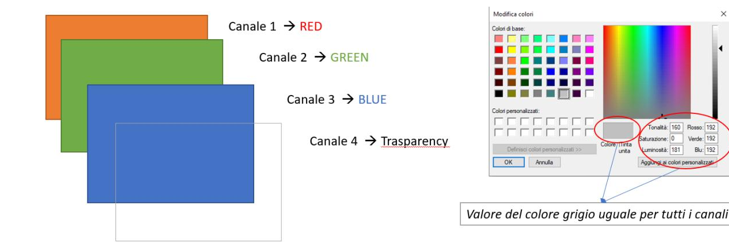
\includegraphics[width=1.2\linewidth]{./immagini/canali.png}}
    \caption{Schema canali RGBA}
    \label{fig:canali}
\end{figure}
	
	Un’immagine viene rappresentata in termini di pixel e sappiamo che:
	\begin{itemize}
		\item Un pixel equivale a 1Byte (ovvero 8 bit);
		\item 1 Byte rappresenta un numero tra 0-255.
	\end{itemize}
	
Quindi, data un’immagine si va creare un buffer di grandezza data da altezza x larghezza x num\_canali, contente il numero totale di bit dell'immagine. A questo punto si va a definire la funzione (vedere in figura … ) che raggruppa i bit di buffer in gruppi da 8, per ottenere i singoli Byte come intero senza segno (questo ci permetterà di non arrotondare il parametro \textbf{ff} all’intero più vicino). \newline
Infine, si con i valori contenuti nel primo canale (Red).
\begin{figure}[H]
    \makebox[\textwidth][c]{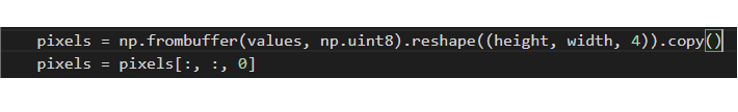
\includegraphics[width=1.3\linewidth]{./immagini/pixels.png}}
    \caption{Funzione pixels}
    \label{fig:pixels}
\end{figure}

Si spiega l’algoritmo nei seguenti passi:
\begin{enumerate}
	\item L’immagine originale viene trasformata in PixMap;
	\item Si definiscono i valori per ogni pixel indicando il canale su cui lavorare;
	\item Setta i valori di \textbf{f} e \textbf{d} immessi dall’utente;
	\begin{enumerate}
		\item Dato F si definisce l’ampiezza dei macro-blocchi;
	\end{enumerate}
	\item Quindi, l’immagine viene divisa in blocchi \textbf{f} di pixels di dimensione \emph{F x F}, partendo dal primo blocco in alto a sinistra;
	\item Per ogni blocco si effettuano le seguenti attività:
	\begin{enumerate}
		\item Si applica la dctn (DCT2 della libreria): \textbf{c = DCT2(f)};
		\item Vengono eliminate le frequenze ckl con k+l >= d;
		\item Si applica idct\textsubscript{n} sulla matrice c: \textbf{ff} = IDCT2(f)
	\end{enumerate}
	\item Trasforma da bit a immagine;
	\item Riporta l’immagine compressa sulla sezione dedicata;
\end{enumerate}
Viene riportata in figura…. Un modello grafico dei passaggi 4 e 5 evidenziando che la ricomposizione dell’immagine non viene effettuata perché una volta finita la compressione sul blocco sarà sostituito direttamente nel blocco occorrente.

\begin{figure}[H]
    \makebox[\textwidth][c]{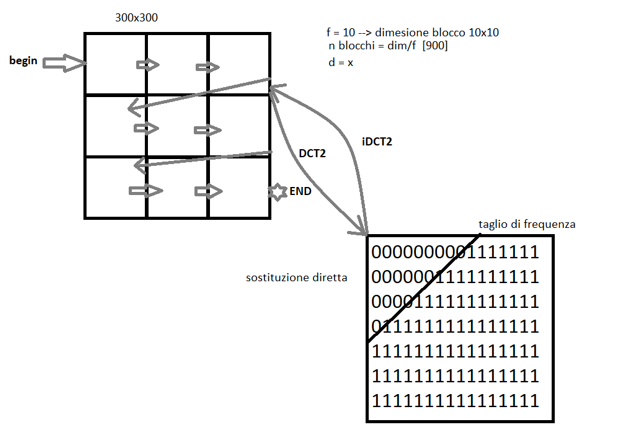
\includegraphics[width=1.3\linewidth]{./immagini/DCT.png}}
    \caption{Schema funzionamento DCT}
    %\label{fig:matlab-memory}
\end{figure}

Di seguito verranno presentati tre esempi di compressione dell’immagine su immagini distinte.\newline
	L'applicazione richiede all’utente di andare a reperire un’immagine cliccando sul bottone “open file” che presenta inizialmente la cartella dove si trova il progetto perché contiene una cartella apposita \path{..\folder\resources} dove può reperire immagini di esempio, ma può anche sceglierne una in locale del suo pc.\newline
	Una volta presa l’immagine va a verificare:
	\begin{enumerate}
		\item Se il formatto è .bmp, altrimenti presenta in messagge-box-error indicando che il formato dell’immagine è sbagliato;
		\item Se l’immagine passata non sia a colori presentando un messagge-box-error indicando che l’immagine deve essere in toni di grigio.
	\end{enumerate}
L’immagine rappresentata contiene una buona qualità di compressione avendo scelto opportunamente i valori \textbf{f} e \textbf{d}. Dalla figura si può notare che sono quasi identiche ma sul contrasto dal colore tutto bianco al colore in tonalità di grigio mostra alcune discrepanze che sono minime visto i valori scelti.

\begin{figure}[H]
    \makebox[\textwidth][c]{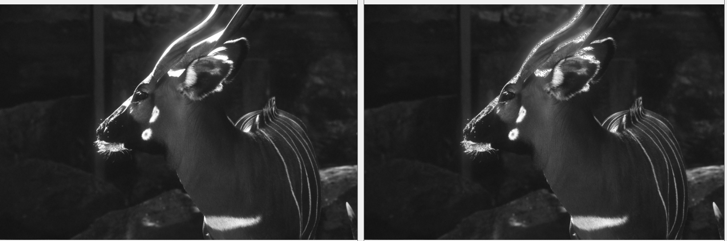
\includegraphics[width=1.3\linewidth]{./immagini/Cervidae.png}}
    \caption{Prima immagine /resources}
    \label{fig: Con f = 124 e d =138}
\end{figure}

L’immagine esposta rappresenta il fenomeno di \textbf{Gibbs} causato dal passaggio del colore nero su bianco e viceversa. Come ben sappiamo, il fenomeno si propaga ed è per questo che sono presenti “cerchi” molto grandi rispetto alle dimensioni dei blocchi f. 
\begin{figure}[H]
    \makebox[\textwidth][c]{
\includegraphics[width=1.3\linewidth]{./immagini/C.png}}
    \caption{Seconda immagine /resources}
    \label{fig: Figura con f = 30 e d = 58}
\end{figure}


\section{Compressione immagine}
	Una volta che viene caricata l’immagine l’utente dovrà definire i valori di F e d in modo tale da studiare la qualità della compressione con diversi esempi che elencheremo alla fine.\newline
	Si spiega l’algoritmo nei seguenti passi:
	\begin{enumerate}
			\item L’immagine originale viene trasformata in formato pixmap;
			\item Si definisce il numero totale di bit in rapporto con il numero di canali (RGBA= 4 canali);
			\item Setta i valori di F e d immessi dall’utente;
				\begin{enumerate}[label=\Alph*]
					\item Dato F si definisce l’ampiezza dei macro-blocchi;
				\end{enumerate}
			\item Quindi l’immagine viene divisa in blocchi f di pixels di dimensione F x F, partendo dal primo blocco in alto a sinistra;
			\item Per ogni blocco si effettuano le seguenti attività:
				\begin{enumerate}[label=\Alph*]
					\item Si applica la dctn (DCT2 della libreria): c = DCT2(f);
					\item Vengono eliminate le frequenze ckl con k+l >= d;	
					\item Si applica idctn sulla matrice c: ff = IDCT2(f)	
				\end{enumerate}
			\item Trasforma da bit a immagine;
			\item Riporta l’immagine compressa sulla sezione dedicata.
	\end{enumerate}

\section{Oservazioni}
	\begin{enumerate}
		\item Le immagini richiedono di lavorare con i 4 tipi di canale: RGBA che in combinazione definiscono il colore.
	\end{enumerate}
	La traccia richiede di lavorare con immagini in toni di grigio, dalle analisi fatte(come in figura in alto a destra) si nota che il valore di \textit{un qualunque grigio} è uguale per tutti i canali.\newline
Di conseguenza si è deciso di lavorare con un solo canale (in questo caso il primo, ovvero Red).
	\begin{enumerate}
		\item Quindi l’immagine viene divisa in blocchi f di pixels di dimensione F x F, partendo dal primo blocco in alto a sinistra;
		\item Per ogni blocco si effettuano le seguenti attività:
		\begin{enumerate}[label=\Alph*]
			\item Si applica la dctn (DCT2 della libreria): c = DCT2(f);
			\item Vengono eliminate le frequenze ckl con k+l >= d;
			\item Si applica idctn sulla matrice c: ff = IDCT2(f)
		\end{enumerate}
	\end{enumerate}
\section{Conclusioni}
L’app di compressione riscontra buoni risultati scegliendo i valori f e d opportuni per l’immagini in toni di grigio mentre per quelle definite solo in due colori ben distinti (black \& white) mostra il fenomeno di Gibbs ma questo succede anche con MatLab.

\end{document}